\documentclass[a4paper]{article}

%% Language and font encodings
\usepackage[english]{babel}
\usepackage[utf8x]{inputenc}
\usepackage[T1]{fontenc}


%% Sets page size and margins
\usepackage[a4paper,top=3cm,bottom=2cm,left=3cm,right=3cm,marginparwidth=1.75cm]{geometry}

%% Useful packages
\usepackage{amsmath}
\usepackage{graphicx}
\usepackage{tabularx} % in the preamble
\usepackage[colorinlistoftodos]{todonotes}
\usepackage[colorlinks=true, allcolors=blue]{hyperref}

\title{Final}
\author{Sami Ellougani}
\date{December 11th, 2017}

\begin{document}
\maketitle

\section{Overview}
We were tasked to choose a dataset that works with Language Modeling with RNNs/LSTMs and figure out with parameters retrieves the lowest perplexity of them all. There were several different observations made as several different parameters were changed, making this final interesting to learn from.

\section{Mark Dataset}
\subsection{Results}

\begin{table}[h!]
\centering
\resizebox{\columnwidth}{!}{
\begin{tabular}{|c c c c c c c c c c c|} 
 \hline
 Batch Size & Learning Rate & Max Grad Norm & Layers & Steps & Hidden Size & Max Epoch & MMax Epoch & Keep Prob & Decay & Test Perplexity \\ [0.5ex]
 \hline
  1 & 1 & 5 & 2 & 20 & 200 & 4 & 13 & 1 & 0.5 & 617 \\
  1 & 1 & 5 & 2 & 20 & 100 & 4 & 13 & 1 & 0.5 & 328 \\
  1 & 0.01 & 5 & 2 & 20 & 200 & 4 & 13 & 1 & 0.5 & 308 \\
  1 & 1 & 5 & 2 & 30 & 200 & 4 & 13 & 0.5 & 0.5 & 207 \\
  1 & 1 & 5 & 2 & 20 & 100 & 4 & 20 & 0.5 & 0.5 & 196 \\
  1 & 1 & 5 & 2 & 20 & 100 & 4 & 13 & 0.5 & 0.25 & 193 \\
  1 & 1 & 5 & 2 & 20 & 100 & 4 & 13 & 0.5 & 0.5 & 192 \\
  1 & 1 & 5 & 2 & 20 & 100 & 8 & 13 & 0.5 & 0.5 & 186 \\
  1 & 1 & 5 & 2 & 20 & 200 & 4 & 13 & 0.5 & 0.75 & 183 \\
  1 & 1 & 5 & 2 & 20 & 200 & 4 & 13 & 0.5 & 0.5 & 152 \\
  \hline
\end{tabular}
}
\end{table}

\subsection{Strategy}
Before I started running several different tests, I went over our labs to gain a better understanding of how Language Modeling with RNNs/LSTMs works. After I gained a better understanding of the network, I learned more about which parameters will affect the network the most. After gaining this understanding, I changed several of those parameters to see which gave the lowest perplexity. 

\subsection{Most Influential Parameter(s)}
The parameters that I found to be the most influential in getting the best results were the learning rate, and the keep probability. The reason why keep probability was so influential is because changing the dropout probability from 1 means that you are addressing the problem of over-fitting. Over-fitting happens when you combine the predictions of many different layers at the same time. Learning rate is influential in almost all networks, but mainly this one as it can not be too low or too high in an effort for the RNN/LSTM to model the language. 

\subsection{Least Influential Parameter(s)}
The parameter that I found to be the least influential was the amount of epochs used within the program. I changed the amount of epochs later on with my best solution, and the perplexity was still the same. The only difference is that the program takes longer to run as it goes through several more epochs. \\ \\ \\

\subsection{Observation}
\begin{figure}[!h]
  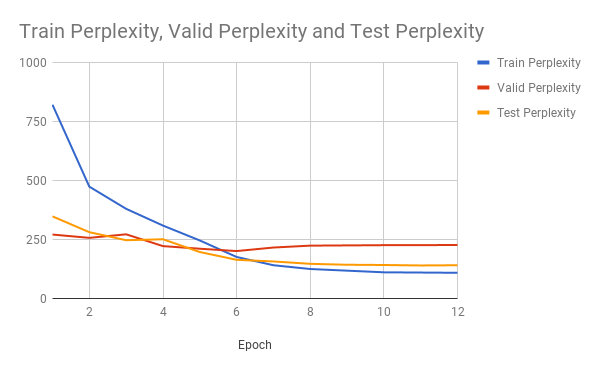
\includegraphics[width=\linewidth]{chart.png}
  \caption{Graph Depicting Varying Perplexities in Epochs}
  \label{fig}
\end{figure}

\subsubsection{Sentence Quality}
The quality of the sentences that this combination of parameters produced were very poor in my opinion. Here is an example of the sentences that this combination of parameters would produce: The crowd to the crowd to the crowd to the crowd to the crowd. As you can tell, this sentence is a poorly constructed sentence.

\subsubsection{Connection between Sentence Quality and Perplexity}
The initial parameters that were loaded into the program gave me a test perplexity of 617. I noticed that this sentence was the most readable of all the sentences in the several different tests I ran. Here is an example of the sentences that were produced from the initial parameters: The stone of the temple was a woman who had been with him, and said, He is not dead for no. As you can see, this sentence is much more constructed than the previous sentence. This showed me that as the test perplexity lowers, so does the quality of the sentence. At one point, I tried running an experiment with 400 hidden units, and I got a test perplexity of 727 with a high quality sentence, proving my theory that lower test perplexity correlates with the lower quality of the sentence.

\end{document}